\documentclass[a4paper,latin,center,onecolumn]{paper} 
\usepackage[english]{babel}
\usepackage{hyperref}

\usepackage[margin=2.5cm]{geometry}
\usepackage{graphicx}
\usepackage{lipsum}
\usepackage{xcolor}
\usepackage{booktabs}

\sectionfont{\large\sf\bfseries\color{black!60!blue}} 
\subsectionfont{\normalsize\sf\bfseries}

\title{ME748: Computer Aided Simulation of Machines}

\subtitle{Assignment 1: Mechanism Selection \\
\hfill
\includegraphics[height=2cm]{Images/Indian_Institute_of_Technology_Bombay_Logo.png}
\vspace{-2cm}}

\author{Madhav Joshi, Roll No - 190110034} 
\institution{Indian Institute of Technology Bombay}


\begin{document}
    \selectlanguage{english}
    % \twocolumn[\maketitle 
    %     \hrule 
    %     \bigskip
    % ]
    \onecolumn\maketitle 
    \hrule 
    \bigskip

    \begin{abstract}
        This is the first assignment of the course ME748, Compurter Aided Simulation of Machines. In this assignment we have to select a mechanism and prepare a report about it. In subsequent term projects we have to do a detailed kinematic and dynamic analysis of this chosen mechanism. Mechanism chosen here is a \it{rice transplanter}.
    \end{abstract}

    \smalltableofcontents

    \section{Mechanism Description} 
        \subsection{Sketch}
            \begin{figure}[hbt!]
                \centering
                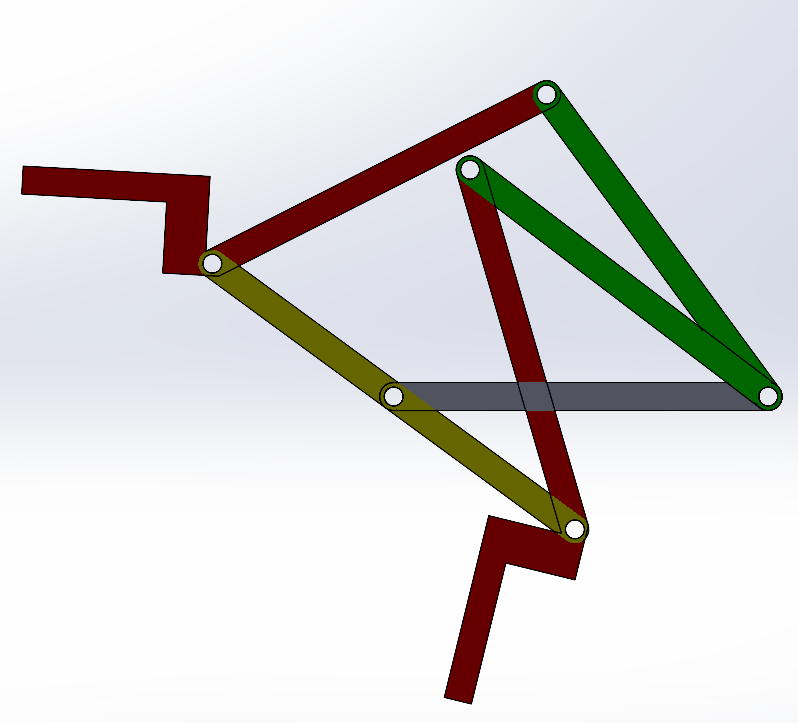
\includegraphics[width=0.9\columnwidth]{Images/Rice_transplanter_1.png}
                \caption{Custom Sketch of Rice transplanter mechanism}
                \label{fig:mySketch}
            \end{figure}
            
            Referring to fig~\ref{fig:mySketch}, the mechanism which I thought about is basically a double 4-bar mechanism working simultaneously and out of phase by 180 deg. The yellow link in the figure is the crank which has couplers attached on both ends. The pistol shaped thing is basically the head which takes the seedlings from the densely grown soil bed placed at the back of the vehicle. The green links are the output links of the 4-bar mechanism which help the head on the coupler maintain its position and orientation to trace a particular trajectory. \par
            But commercially, non circular gear based mechanisms are used, due to which the size of the mechanism is reduced considerably. 
            \begin{figure}[hbt!]
                \centering
                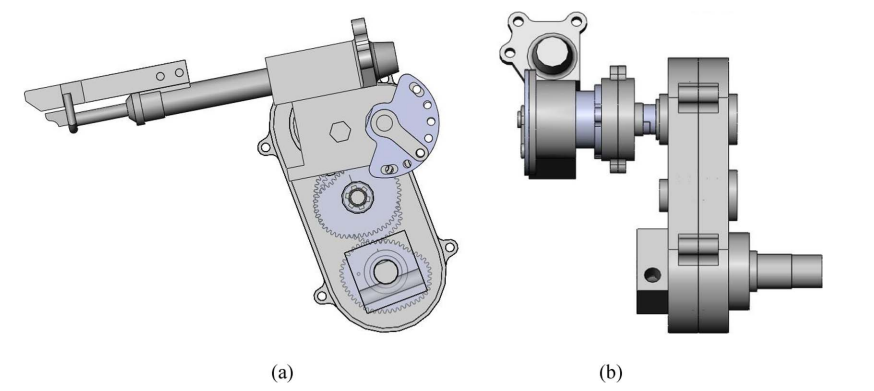
\includegraphics[width=0.9\columnwidth]{Images/side_view_pot_seedling_transplanter.png}
                \caption{Side views of 3D model of Pot Seedling Transplanter mechanism: (a) front view and (b) lateral view}
                \label{fig:refSketch}
            \end{figure}

            Referring to fig~\ref{fig:refSketch} from paper \cite{camPST} on Pot Seedling Transplanter (PST), we can see that the construction of the mechanism is done using non circular gears, which also provide the advantage of simple installation, protection from external environment and reduction in material cost.
        
        \subsection{Description}
            A rice transplanter is a specialized transplanter fitted to transplant rice seedlings onto paddy field. There are mainly two types of rice transplanters, riding type and walking type. Riding type is power driven and can usually transplant six lines in one pass. On the other hand, walking type is manually driven and can usually transplant four lines in one pass. But both of them are costly so many consumers transplant manually. If we transplant rice manually, it takes a lot of time to plant large number of plants. So we use mechanical transplanting machine. Mechanical transplanting of rice is the process of transplanting young rice seedlings, which have been grown in a mat nursery, using a self-propelled rice transplanter. \par
            
            Here, riding type transplanter mechanism has been chosen for the assignment and subsequent term projects. There is mainly one crank or rotating gear which keeps the relative trajectory of the end effector fixed.

        \subsection{Application}
            Apart from transplanting rice seedlings, this mechanism can also be used to transplant other kind of seedlings with small modifications. In rice plantation, a significant 30\% of the time is taken up to transplant the rice seedlings. This riding type transplanter drastically improves the speed. Rice is the most important cereal food crop of India, it occupies about 23.3\% of the gross cropped area of the country and plays an important role in national food grain supply. Thus approximately 23.3\% cultivated land used for growing rice.
        
    \section{Context of Use} 
        \subsection{History}
            In the early 1950s, Japanese company Kubota started the development of rice transplanter. In 1968, they launched world's first 2-row walk behind rice transplanter. Slowly it was being mass manufactured. Then came 6-row ride-on rice transplanter in 1976. Subsequently rice planters started coming with row-side fertilizer applicator to reduce amount of applied fertilizer and prevent water contamination. Pesticide spraying and other simultaneous features also subsequently developed. Thus weight to power ratio significantly reduced from 57.1 (kg/PS) in 1980s to 38.3 (kg/PS) in 2000s.
        
        \subsection{Evolution and Alternate Mechanisms}
            Two alternate mechanisms are shown in fig~\ref{fig:mySketch} and fig~\ref{fig:refSketch}. There have been many research papers regarding the design of just the end effector of the mechanism for efficient removal of seedlings from mats procured from nursery. \par

            The evolution of mechanism has been mainly from walk behind manual transplanter to ride on automatic transplanters with many features combined. Namely, transplanting, fertilizing, ground levelingm pesticide and herbicide spraying.

            \begin{figure}[hbt!]
                \centering
                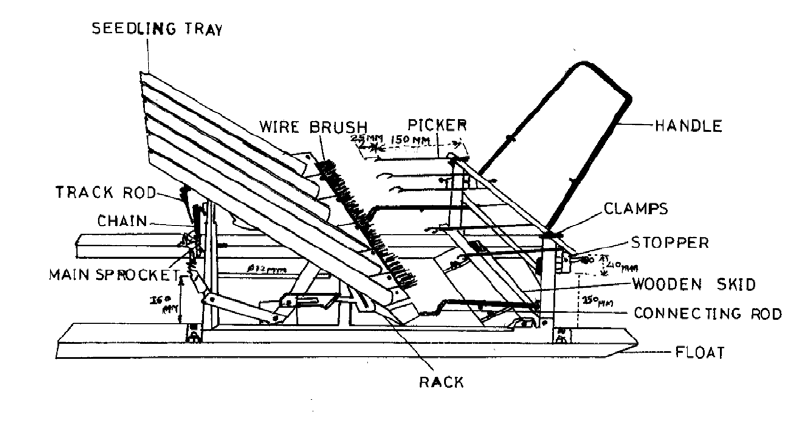
\includegraphics[width=0.9\columnwidth]{Images/Six-row-manually-operated-paddy-transplanter.png}
                \caption{6-row manually operated paddy transplanter}
                \label{fig:manualTransplanter}
            \end{figure}

            \begin{figure}[hbt!]
                \centering
                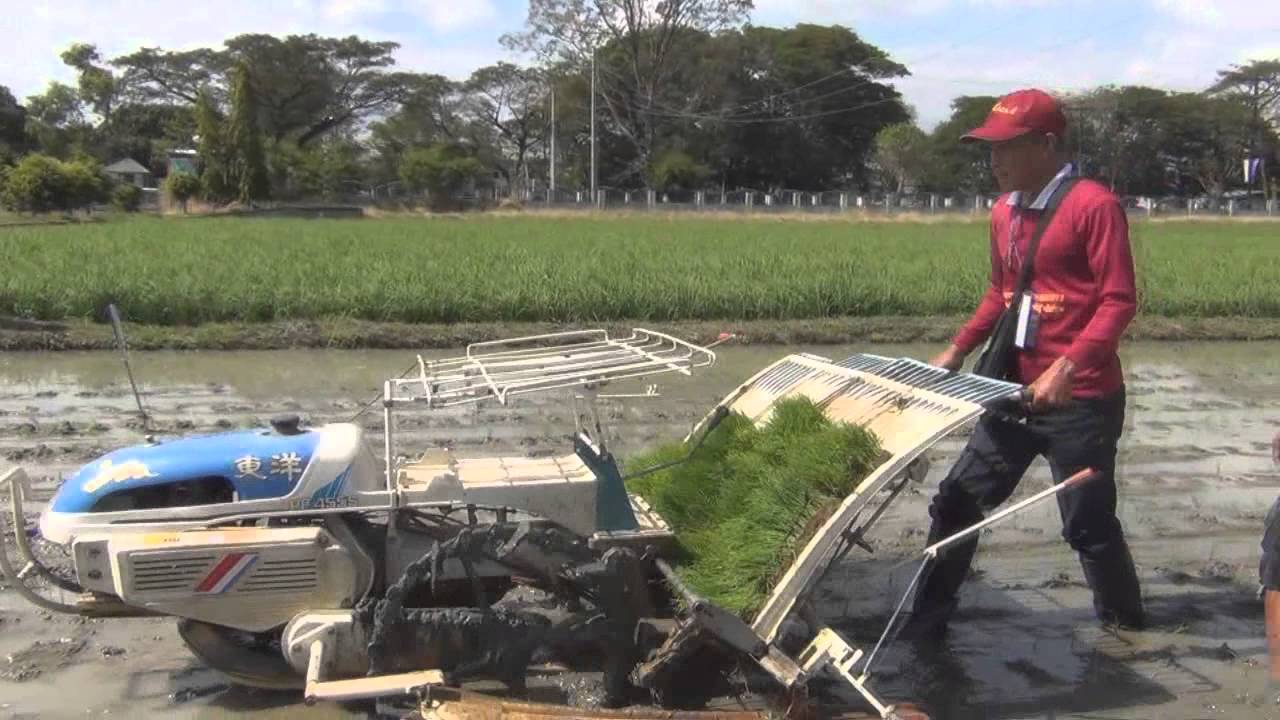
\includegraphics[width=0.9\columnwidth]{Images/walk_behind_transplanter_new.jpg}
                \caption{New walk behind transplanter}
                \label{fig:walkBehindTransplanter}
            \end{figure}

            \begin{figure}[hbt!]
                \centering
                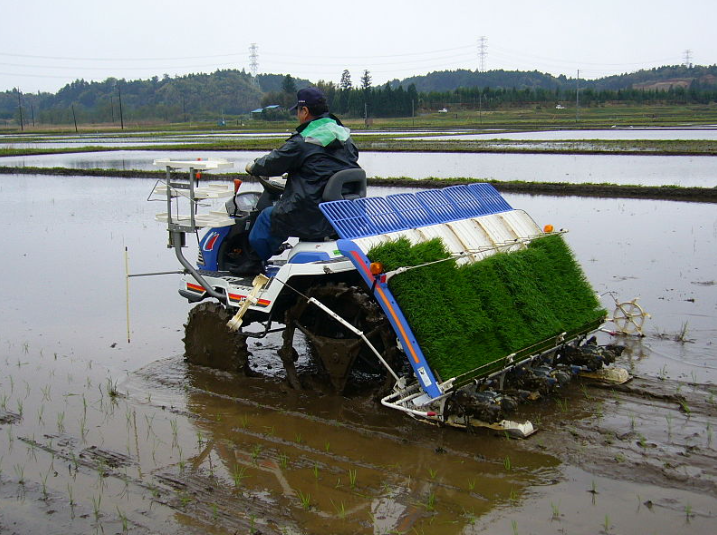
\includegraphics[width=0.9\columnwidth]{Images/ride_on_transplanter_new.png}
                \caption{New ride on transplanter}
                \label{fig:rideOnTransplanter}
            \end{figure}

            \begin{figure}[hbt!]
                \centering
                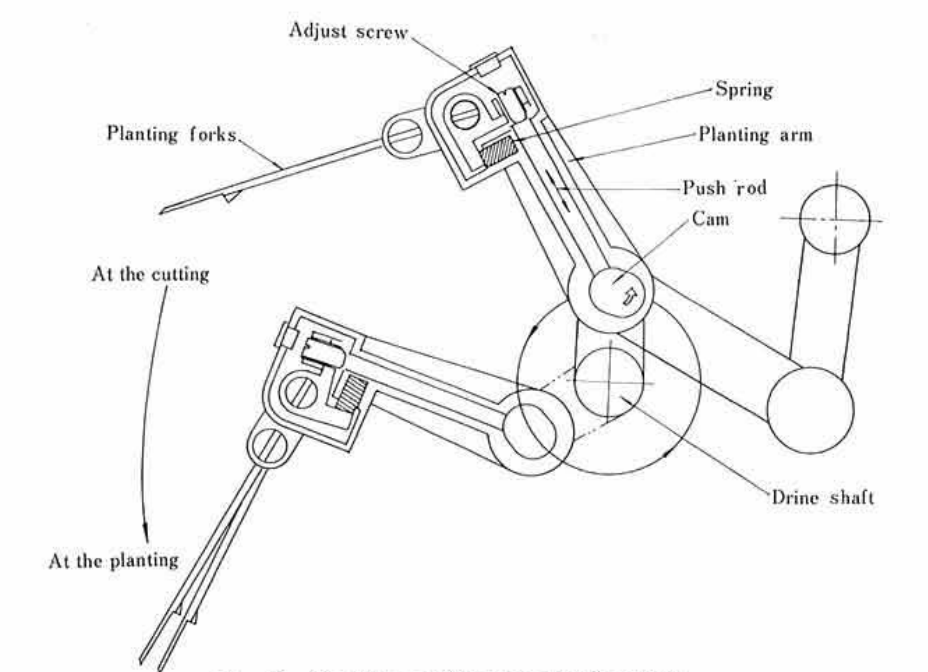
\includegraphics[width=0.9\columnwidth]{Images/seedling_cutting_by_planting_fork.png}
                \caption{A single 4-bar transplanter}
                \label{fig:4barTransplanter}
            \end{figure}

            The transplanter can have double 4-bar linkage as shown in fig~\ref{fig:mySketch} or a single 4-bar to reduce cost and if faster transplantation is not possible as shown in fig~\ref{fig:4barTransplanter}.

    \section{Kinematics}
        \subsection{Kinematic Sketch}

        The kinematic sketch of a self propelled transplanter is shown in fig~\ref{fig:kineSketch} and its original counter part is show in fig~\ref{fig:originalMechanism}. The sketch of rear part of transplanter is shown in fig~\ref{fig:refSketch}.

        \begin{figure}[hbt!]
            \centering
            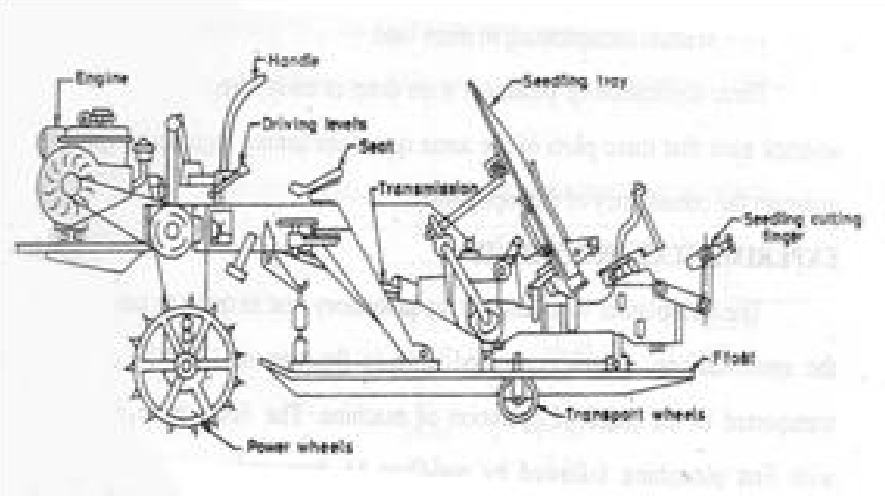
\includegraphics[width=0.9\columnwidth]{Images/Kinematic_sketch_self_propelled_transplanter.png}
            \caption{Kinematic Sketch of a self propelled riding type transplanter}
            \label{fig:kineSketch}
        \end{figure}

        \begin{figure}[hbt!]
            \centering
            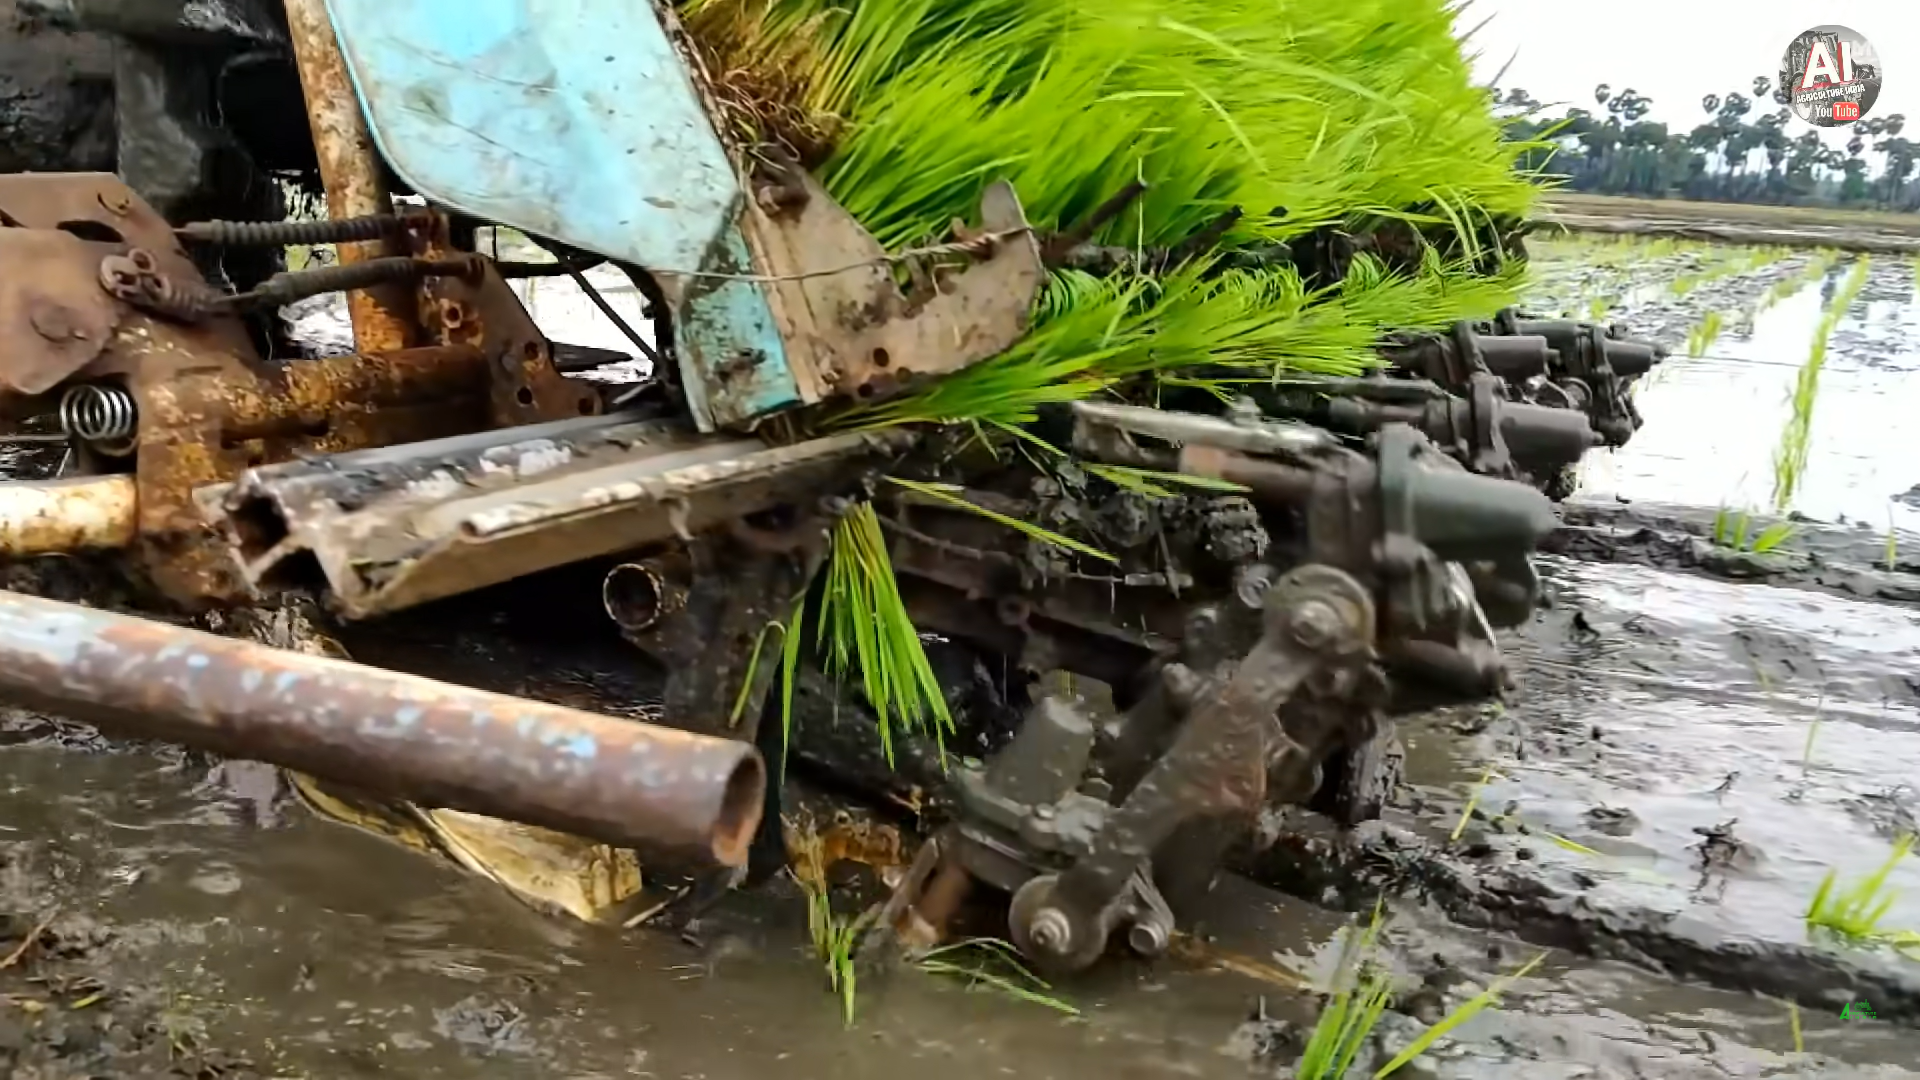
\includegraphics[width=0.9\columnwidth]{Images/Original_transplanter.png}
            \caption{Rear view of actual transplanter mechanism}
            \label{fig:originalMechanism}
        \end{figure}
        
        \subsection{Description of Motion Transmission}
            Motion transmission is done using non circular gears, which are designed based on constraints governed by the angle of the nursery mat, velocity with which we can pull the seedling and the trajectory it should follow while planting the seedling.

        \subsection{Expected Displacement Profile}
            Expected displacement profile of the mechanism is shown in fig~\ref{fig:dispPro1} and fig~\ref{fig:dispPro2}.

            \begin{figure}[hbt!]
                \centering
                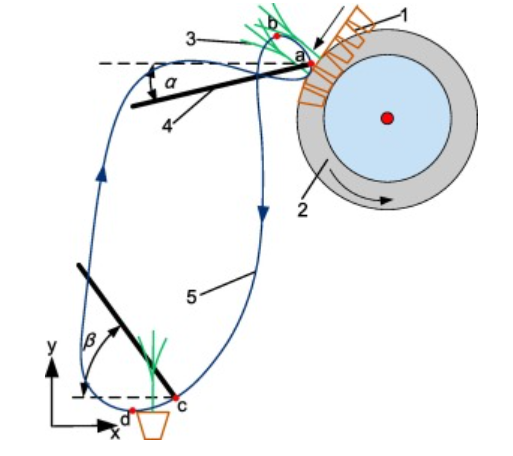
\includegraphics[width=0.9\columnwidth]{Images/displacement_profile_1.png}
                \caption{Displacement profile wrt the vehicle}
                \label{fig:dispPro1}
            \end{figure}

            \begin{figure}[hbt!]
                \centering
                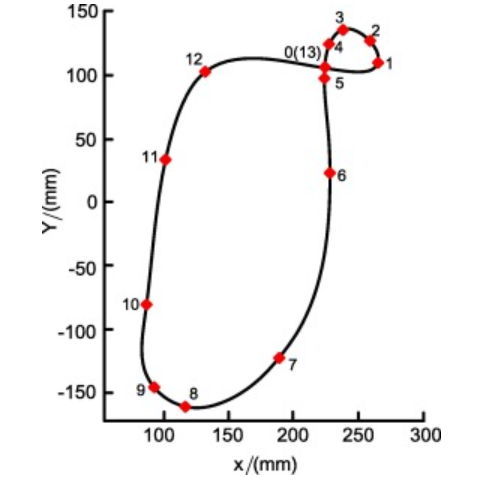
\includegraphics[width=0.9\columnwidth]{Images/displacement_profile_2.png}
                \caption{Displacement profile coordinates}
                \label{fig:dispPro2}
            \end{figure}


        \subsection{Expected Velocity Profile}
            Expected time dependent height and angle graph is shown in the fig~\ref{fig:angleHeight}. Taking a derivative of which would give us velocity profile.

            \begin{figure}[hbt!]
                \centering
                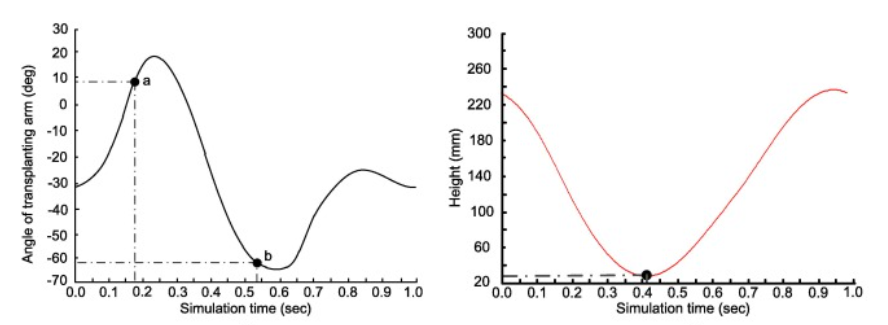
\includegraphics[width=0.9\columnwidth]{Images/height_and_angle_wrt_time.png}
                \caption{Angle and height variation wrt time}
                \label{fig:angleHeight}
            \end{figure}

        \subsection{Expected Acceleration Profile}
            The transmission ratio variation is shown in fig~\ref{fig:transmissionRatio}.
            
            \begin{figure}[hbt!]
                \centering
                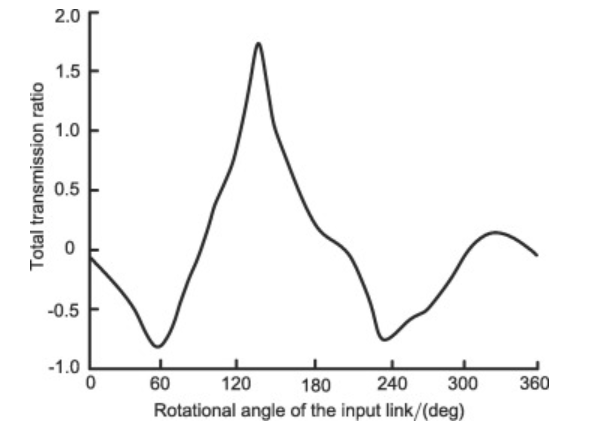
\includegraphics[width=0.9\columnwidth]{Images/transmission_ratio.png}
                \caption{Variation of transmission ratio wrt rotational angle of input link}
                \label{fig:transmissionRatio}
            \end{figure}
        
    \section{Dynamics} 
        \subsection{Expected speed of operation}
            Expected rotational speed of axel or crank is around 90 rpm. 

        \subsection{Possible problems with extreme speeds}
            Lower speed would consume more time and hence more fuel, whereas for the higher speed, the literature has reported significant misplantation, close to 20\% for speeds of 120 rpm whereas it is only 5\% for 90 rpm.

    \begin{thebibliography}{999}

        \bibitem{camPST}
            Liang Sun, Xuan Chen, Chuanyu Wu, Guofeng Zhang, Yadan Xu, 
            \emph{Synthesis and design of rice pot seedling transplanting mechanism based on labeled graph theory},
            Computers and Electronics in Agriculture,
            Vol. 143,
            2017,
            Pages 249-261,
            ISSN 0168-1699,
            \href{https://doi.org/10.1016/j.compag.2017.10.021}{https://doi.org/10.1016/j.compag.2017.10.021}
            
        \bibitem{6rowManuallyOperatedTransplanter}
            Yadav, Dr \& Mital, Patel \& P, Shukla \& Pund, Sahastrarashmi. (2007). \emph{Ergonomic evaluation of manually operated six-row paddy transplanter.} International Agricultural Engineering Journal. 16. 147-157. 
        
        \bibitem{selfPropelled}
            Guru, Prabhat \& Chhuneja, Naresh \& Dixit, Anoop \& Tiwari, Prem \& Kumar, Anjani. (2018). \emph{Mechanical transplanting of rice in India: Status, technological gaps and future thrust.} ORYZA- An International Journal on Rice. 55. 10.5958/2249-5266.2018.00012.7. 
        
    \end{thebibliography}

\end{document}